\chapter{Decentralized Applications}\label{chapter::decentralizedapps}

	\section{Introduction}
	An Application software or \textit{app} is a computer program designed to perform a specific set of tasks or actions for the end user. There are countless number of applications in use today and the majority of them are web applications following a centralized client-server model\cite{raval2016decentralized}.
	
	\begin{figure}[h]
		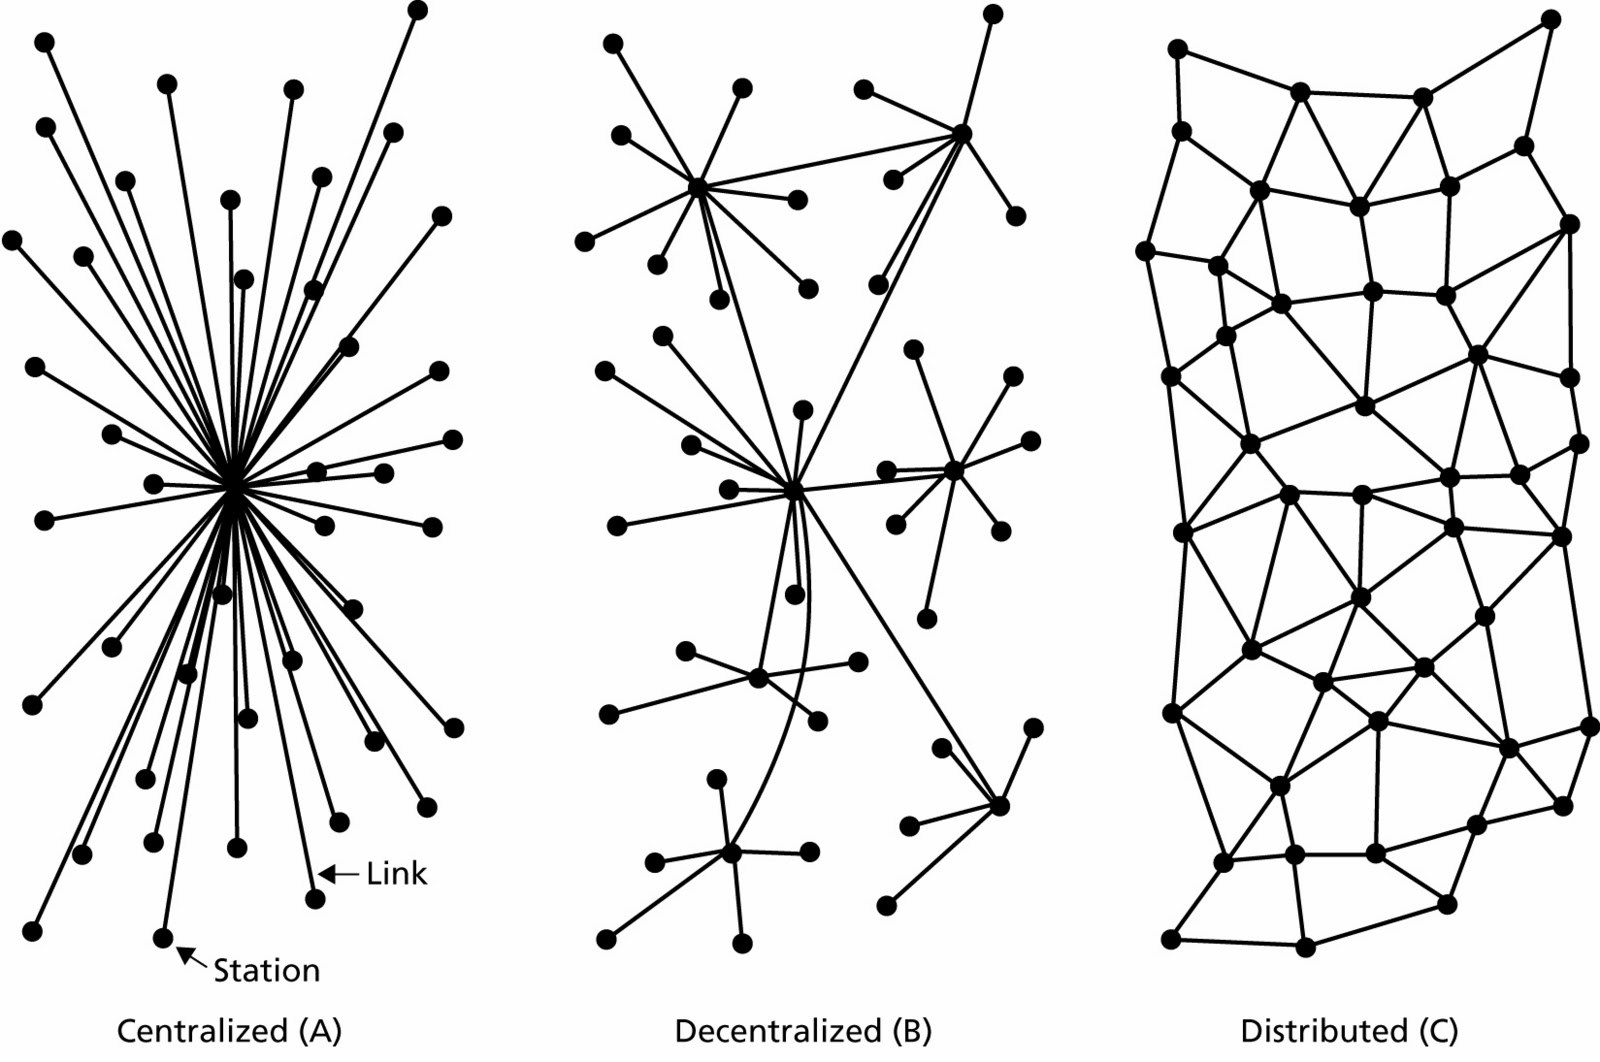
\includegraphics[width=\linewidth]{figures/network-models}
		\caption{\label{fig:applications} The three way of modeling web applications}
	\end{figure}
	
	Figure~\ref{fig:applications} shows a visual representation of three different ways of modeling web applications\cite{baran1964distributed}. Here, \textit{Centralized} and \textit{Decentralized} refers to level of control, while \textit{Distributed} refers to differences of location. Both centralized and decentralized systems can be distributed as well.
	
	\subsection{Centralized}
	It's currently the widespread way of building software applications. In this model a central server control the flow of information and governs the operation of individual units. Since the control is centralized, these types of systems suffer from single point of failure risk.
	
	\subsection{Distributed}
	In a Distributed model, the control still resides with a central server, however, the computation is spread across multiple nodes or servers.
	
	\subsection{Decentralized}
	In a Decentralized model, there is no central point of control as it's spread across all the servers running the application. Applications built using this model do have a single point of failure and are inherently fault tolerant.

\section{Enabling Technologies and Concepts}

	\subsection{Data}
	
	\subsection{Identity}
	
	\subsection{Value}
	
	\subsection{Computing}
	
	\subsection{Bandwidth}